% Inbuilt themes in beamer
\documentclass{beamer}


%Defining some colours
\definecolor{darkred}{rgb}{0.8,0,0}

% Theme choice: there a number of preset themes to choose from
% Play around with them, Cambridge is nice for first pres
%\usetheme{Szeged}
\usetheme{CambridgeUS} %setting the main theme
%\usecolortheme{beaver} % setting colour theme
\usefonttheme{professionalfonts} %font theme
\useinnertheme[shadow=true]{rounded}
%\useoutertheme{} %outer theme

%\setbeamertemplate{footline} %Remove footer line in all slides
\setbeamertemplate{navigation symbols}{} %removes navigation symbols
\setbeamertemplate{footline}[page number] %removes footer line, keeps pg#
\setbeamertemplate{caption}{\insertcaption} 

%Setting colours for boxes and captions
\setbeamercolor{block title}{bg=darkred, fg=white}
\setbeamercolor{block body}{bg=darkred!10}

% For the Flowchart
\usepackage{tikz}
\usetikzlibrary{shapes.geometric, arrows}
\tikzstyle{startstop} = [rectangle, rounded corners, minimum width=3cm, minimum height=1cm,text centered, draw=black, fill=red!30]
\tikzstyle{process} = [rectangle, minimum width=3cm, minimum height=1cm, text centered, draw=black, fill=orange!30]
\tikzstyle{decision} = [diamond, minimum width=3cm, minimum height=1cm, text centered, draw=black, fill=green!30]
\tikzstyle{arrow} = [thick,->,>=stealth]


% Title page details: 
\title[BEAP Dec 2022]{Estimating Evolutionary Parameters for Protein Low Complexity Regions using an Approximate Bayesian Computation} 
\author{Alexander Turco}
\date{\today}
\logo{
\includegraphics[height=1cm, width=1cm]{logo.png}}

% Bibliography stuff
\usepackage[natbib=true, sorting=nyt, style=authoryear-comp]{biblatex}
\addbibresource{ABC1.bib}

%Extra packages
\usepackage{makecell}

%For itemize
\setbeamertemplate{itemize item}[triangle]



\begin{document}
	
	% For my introduction slides, there will be the slide with my title and name as well as an outline slide with the brief overview of what I will discuss.
	% Title page frame - SLIDE 1%%%%%%%%%%%%%%%%%%%%%%%%%%%%%%%%%%%%%%%%%%%%%%%%%%%%%%%%%%%%%%%%%%%%%%%%%%%%%%%%%%%%%%%%%%%%%%%%%%%%%%%%%%%%%%%%%%%%%%%%%%%%%%%%%%%%
	\section{Introduction}
	\begin{frame}
		\titlepage 
	\end{frame}
	
	% Remove logo from the next slides
	\logo{}
	
	% Outline frame - SLIDE 2
	\begin{frame}{Overview}
		
		\begin{center}
		\begin{minipage}{6cm}
				
		  		\begin{block}{} \hyperlink{link1}{Background information} \end{block}
		  		\begin{block}{} Research Questions/Explorations \end{block}
		  		\begin{block}{} Experimental Approach \end{block}
		  		\begin{block}{} Results \end{block}
		  		\begin{block}{} Conclusion and Future Work \end{block}

		\end{minipage}
		\end{center}
	
	\end{frame}
	
	% For my Background slides, I will talk about important things such as WHat LCRs are, their evolution, stuff like that
	% SLIDE 3 - WHAT ARE LCRs%%%%%%%%%%%%%%%%%%%%%%%%%%%%%%%%%%%%%%%%%%%%%%%%%%%%%%%%%%%%%%%%%%%%%%%%%%%%%%%%%%%%%%%%%%%%%%%%%%%%%%%%%%%%%%%%%%%%%%%%%%%%%%%%%%%%%%
	% The graphic for this slide is an image of some output from segA with the parameters in the brackets
	\section{Background}
	\begin{frame}{What are LCR's?}
		\label{link1}
		
		\begin{block}{\textit{Saccharomyces cerevisiae} SRP40 Protein LCRs}
			$>$CAA82171.1(25-125) complexity=0.92 (15/1.90/2.20)
			sssssssssssssssssssssssssgessssssssssssssdssdssdsessssssssss
			ssssssdsesssesdssssgsssssssssdesssesesede \newline
			
			$>$CAA82171.1(149-282) complexity=1.33 (15/1.90/2.20)
			esssssessssgsssssesesgsesdsdsssssssssdsesdsesdsqssssssssdsss
			dsdssssdsssdsdssssssssssdsdsdsdsssdsdssgssdsssssdsssdestssds
			sdsdsdsdsgssse \newline
			
			$>$CAA82171.1(298-316) complexity=2.18 (15/1.90/2.20)
			tpassnestpsasssssan
			
		\end{block}		
		
	\end{frame}

	% SLIDE 4 - I do Not Know if I am including this slide
	% The Graphic for this slide is an  
	% Entropy, which is measured by Shannon's Entropy equation is a measure of compositional complexity which uses the proportion of residue(s)
	% in a subsequence to measure the compositional state of that subseequence - A lower variety of residues = lower entropy 
	\begin{frame}{Shannon's Entropy - MAYBE }
		
			$H = -L\sum p_i log_2(p_i)$
		
	\end{frame}

	%SLIDE 5 - LCR's PRESENT IN UNIQUE WAYS
	\begin{frame}{LCR's Present in Unique Ways }
		
		\begin{alertblock}{Homorepeats}
			Consecutive iterations of a single residue
		\end{alertblock}
	
		\begin{center}
			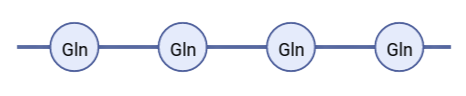
\includegraphics[width=5cm, height=1cm]{poyglut.png}
		\end{center} \pause
	
		\begin{alertblock}{Direpeats}
			Consecutive iterations of two ordered, different residues
		\end{alertblock}
	
		\begin{center}
			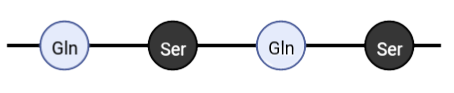
\includegraphics[width=5cm, height=1cm]{direpeat.png}
		\end{center} \pause

		\begin{alertblock}{Tandem Repeats}
			Sequence of residues which are repeated a number of times
		\end{alertblock}
	
		\begin{center}
			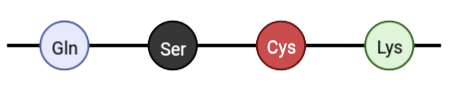
\includegraphics[width=5cm, height=1cm]{tandem.png}
			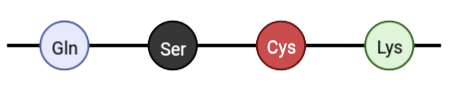
\includegraphics[width=5cm, height=1cm]{tandem.png}
		\end{center}
	
	\end{frame}

	%SLIDE 6 LCRs are hypermutable
	% Maybe change the lines from the fly to dashed - as per photo Lauren Sent
	\begin{frame}{LCR's are Hypermutable }
		
		
		\begin{center}	
		
\includegraphics[width=8cm, height=3cm]{drosophila.png}
		\end{center}
	
		\begin{center}	
		\begin{tabular}{|cccc|}
			\hline
			\makecell{\textbf{mam} \\ \textbf{domain}} & \textbf{Size (bp)} & \makecell{\textbf{Amino Acid} \\ \textbf{Substitutions}} & \makecell{\textbf{Amino Acid/} \\ \textbf{Total Substitutions}}  \\ 
			\hline
			Unique & 933 & 26 & 0.15\\ 
			\hline
			Repetitive & 810 & 47 & 0.42\\ 
			\hline
		\end{tabular}\newline\newline
		\end{center}
	
	%\footer{\tiny\citep{newfeld1991interspecific}}
	\footnotetext[1]{\tiny\cite{newfeld1991interspecific}}	
	\end{frame}

	%SLIDE 7 - Mechanisms of LCR Evolution
	\begin{frame}{Proposed Mechanisms of LCR Evolution}
		\textit{1. Polymerase Slippage/Slipped Strand Mispairing}
		\begin{columns}
			
			\column{0.5\textwidth}
			\centering
			\begin{figure}
				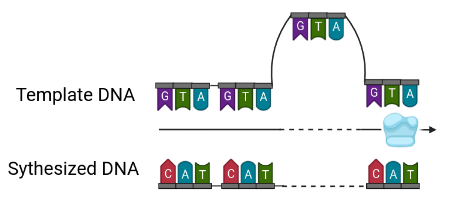
\includegraphics[width=\columnwidth, height=2.5cm]{slippage2.png} \\~\\
				\caption{\centering \textbf{Polymerase Slips Forward}}
			\end{figure}
			
			\column{0.5\textwidth}
			\centering
			\begin{figure}
				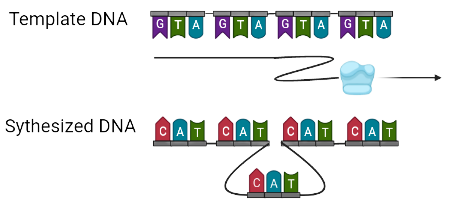
\includegraphics[width=\columnwidth, height=2.5cm]{slippage1.png} \\~\\
				\caption{\centering \textbf{Polymerase Slips Backwards}}
			\end{figure}
		
		\end{columns}
	
	\footnotetext[2]{\tiny\cite{levinson1987slipped,sehn2015insertions}}
	\end{frame}

	%SLIDE 8 - Mechanisms of LCR Evolution
	\begin{frame}{Proposed Mechanisms of LCR Evolution}
		\textit{2. Unequal Recombination} \newline\newline
		
		\begin{figure}
			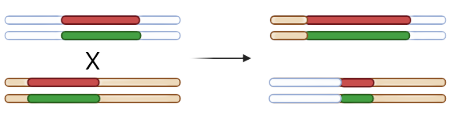
\includegraphics[width=8cm, height=1.8cm]{unequal.png} \\~\\
		\end{figure}
		
	\footnotetext[3]{\tiny\cite{levinson1987slipped,sehn2015insertions}}	
	\end{frame}
	
	%SLIDE 8 - Why Care About LCR Evolution?
	\begin{frame}{Why Care about LCRs and Their Evolution? }
	
	\begin{center}	
		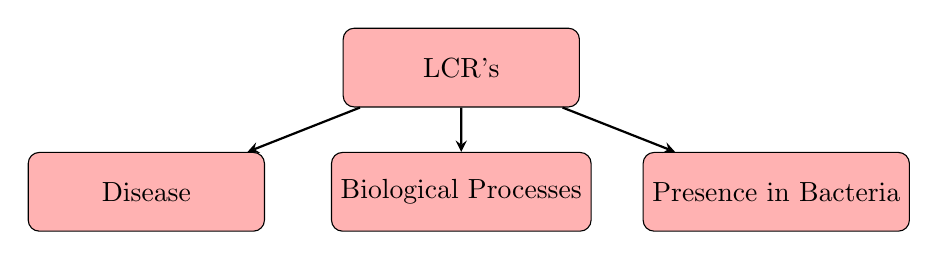
\begin{tikzpicture}[node distance=2cm]
			\node[startstop] (1) {Disease};
			\node[startstop, right of=1, xshift=2cm] (2) {Biological Processes};
			\node[startstop, right of=2, xshift=2cm] (3) {Presence in Bacteria};
			\node[startstop, above=2, xshift=4cm, yshift=1cm] (4) {LCR's};
			
			\draw [arrow] (4) -- (1);
			\draw [arrow] (4) -- (2);
			\draw [arrow] (4) -- (3);
			
		\end{tikzpicture}
	\end{center}

		\begin{columns}
			
			\column{0.33\textwidth}
			\centering
			\begin{figure}
				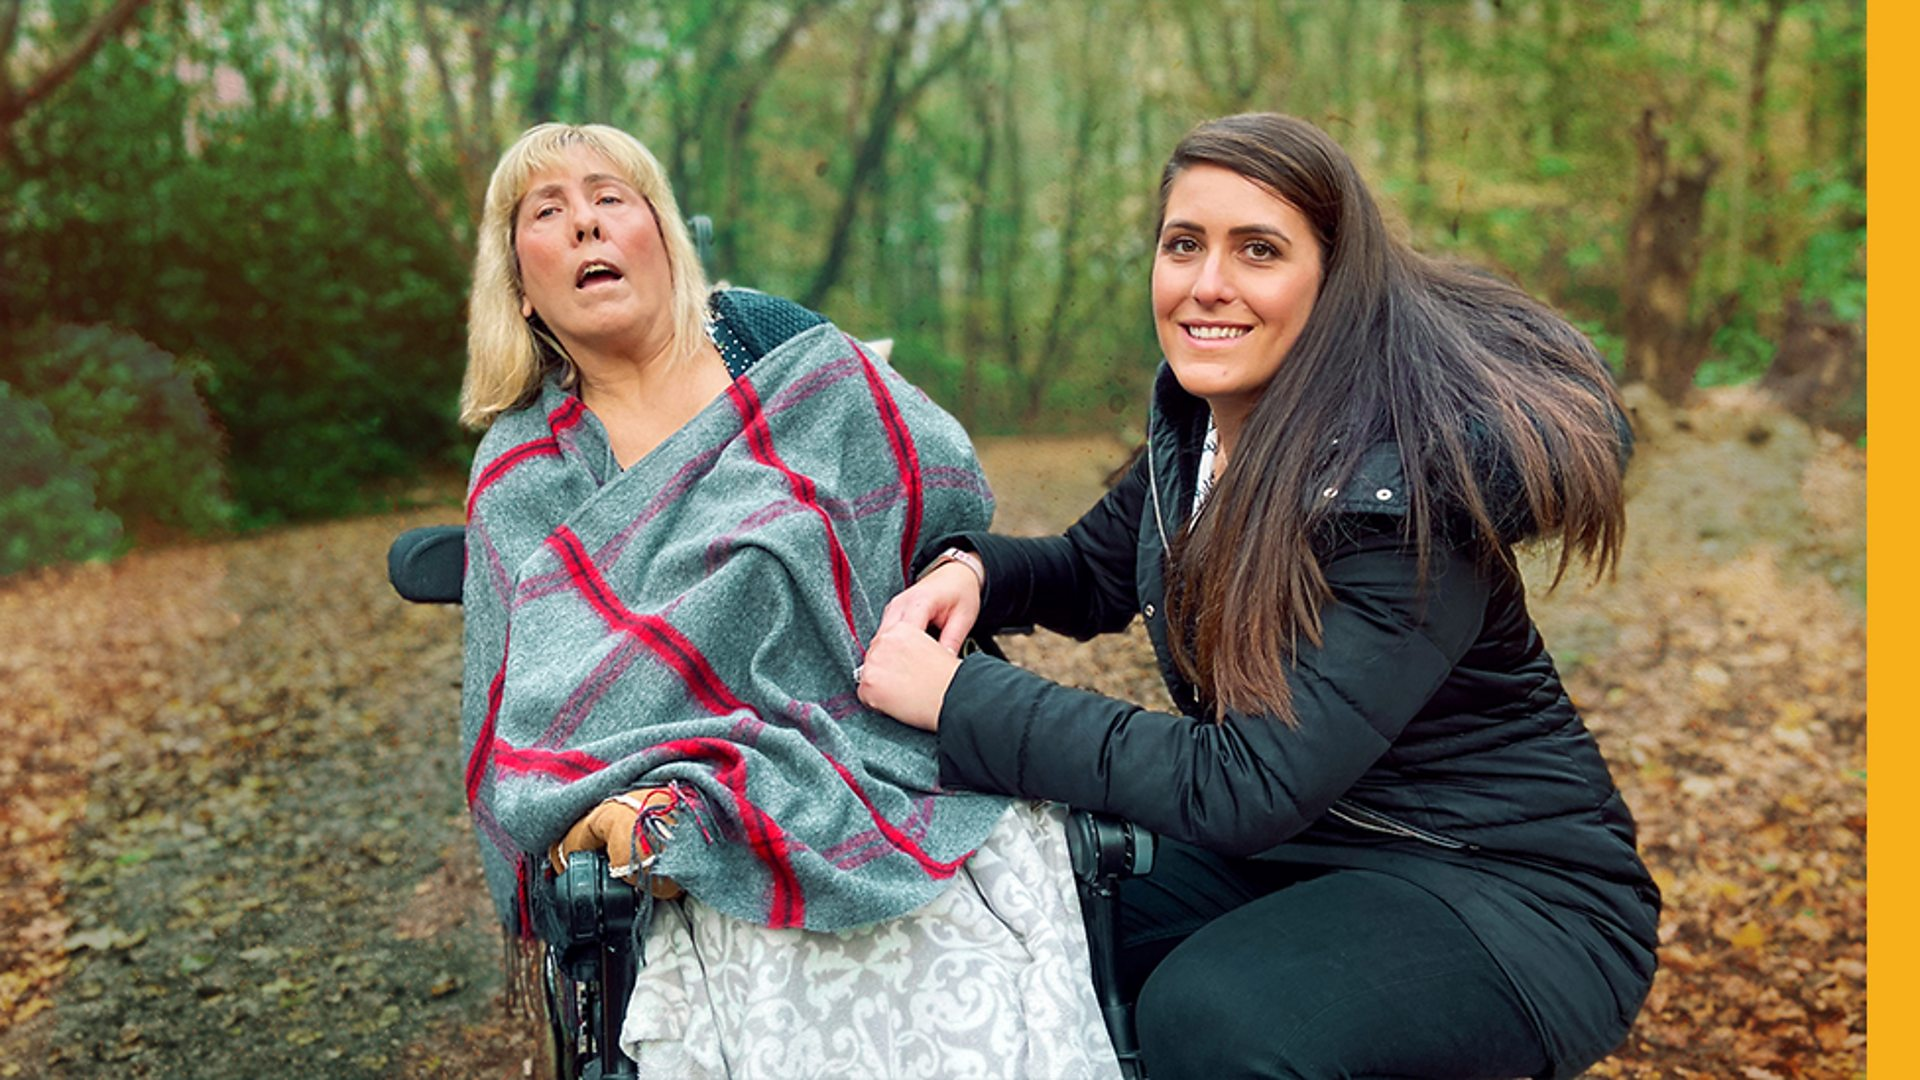
\includegraphics[width=\columnwidth, height=2.5cm]{huntington.jpg} \\~\\
				\caption{\centering \textit{Huntington's Disease}}
			\end{figure}
			
			\column{0.33\textwidth}
			\centering
			\begin{figure}
				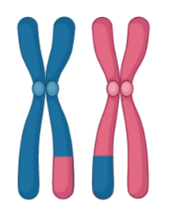
\includegraphics[width=2.5cm, height=2.5cm]{chrom.png} \\~\\
				\caption{\centering \textit{Genetic Recombination}}
			\end{figure}
		
			\column{0.33\textwidth}
			\centering
			\begin{figure}
				\vspace{-0.4cm}
				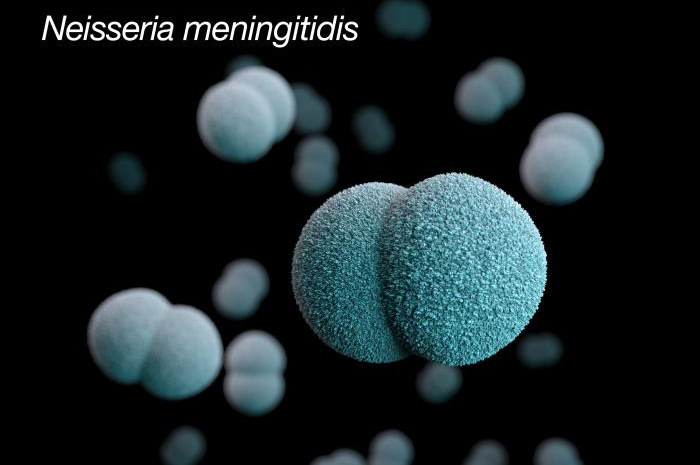
\includegraphics[width=\columnwidth, height=2.5cm]{menin.jpg} \\~\\
				\caption{\centering \textit{Neisseria meningitidis}}
			\end{figure}
			
		\end{columns}
	
	\end{frame}

	%For my Research questions/Exploration slides, I will talk about things such as
	%SLIDE 9%%%%%%%%%%%%%%%%%%%%%%%%%%%%%%%%%%%%%%%%%%%%%%%%%%%%%%%%%%%%%%%%%%%%%%%%%%%%%%%%%%%%%%%%%%%%%%%%%%%%%%%%%%%%%%%%%%%%%%%%%%%%%%%%%%%%%%%%%%%%%%%%
	\section{Research Questions/Exploration}
	
	\begin{frame}{What will this Study Explore?}
		\begin{itemize}
			\item Estimation of evolutionary parameters (mutation rate, indel rates) \newline
			\item Various models of insertions and deletions \newline
			\item Summary statistics which best explain data
		\end{itemize}
		
	\end{frame}

	%For my Experimental approach slides, I will talk about things such as 
	%SLIDE 10%%%%%%%%%%%%%%%%%%%%%%%%%%%%%%%%%%%%%%%%%%%%%%%%%%%%%%%%%%%%%%%%%%%%%%%%%%%%%%%%%%%%%%%%%%%%%%%%%%%%%%%%%%%%%%%%%%%%%%%%%%%%%%%%%%%%%%%%%%%%%%%%%%%%
	\section{Experimental Approach}
	\begin{frame}{What Approach will be Taken?}
	
	
	\end{frame}

	%SLIDE 11
	\begin{frame}{Why use an ABC-MCMC}
	
	
	\end{frame}

	%Slide 12 - Here put the ABC-MCMC algorithm described by Marjoram (one Brian used in his MCMC slides)
	\begin{frame}{MCMC for ABC}
		
		\begin{enumerate}
			\item Propose a move from $\theta$ to $\theta'$ according to a transition kernel $q(\theta,\theta')$.
			\item Generate simulated dataset $D'$ using $\theta'$ and calculate $S'$.
			\item If $\rho(S', S) \le \epsilon$ continue to 4, otherwise remain at $\theta$ and go to 1.
			\item Calculate \newline \begin{center}$\alpha(\theta, \theta') = min(1, \frac{\pi(\theta')q(\theta',\theta)}{\pi(\theta)q(\theta, \theta')})$ \end{center}
			\item Accept $\theta'$ with probability $\alpha$, otherwise stay at $\theta$.
			\item Return to 1.
		\end{enumerate}
	
		\footnotetext[3]{\tiny\cite{marjoram2003markov}}	
	\end{frame}

	%Slide 13 - Here we put MY version of the algorithm - We could also put these on the same slide and just compare! SLIDE 14 AND 15
	%Should I put the equation for calculating distance in this slide? or at the end in the appendix idk yet.
	\begin{frame}{MCMC for ABC: Modified Algorithm}
	
		\begin{enumerate}
			\item Propose a move from $\theta$ to $\theta'$ according to the normal distribution \pause
			\item Create a random protein sequence and mutate over many generations using $\theta'$ to generate simulated Dataset $D'$ \pause
			\item Calculate summary statistics for simulated dataset $D'$ \pause
			\item If $d(S',S) \le \epsilon$, go to next step, otherwise stay at $\theta$ and return to 1 \pause
			\item Accept $\theta'$ with probability ?? Ask Brian ab this again lol \pause
			\item Return to step 1
		\end{enumerate}
	
	\end{frame}

	%Slide 14 - Maybe to this slide - Maybe throw in extra slides for reference
	\begin{frame}{Simulation Step - MAYBE}
	
	
	\end{frame}

	%For my Results slides, I will talk about things such as the results I have, But i don't have any right now
	%SLIDE 15%%%%%%%%%%%%%%%%%%%%%%%%%%%%%%%%%%%%%%%%%%%%%%%%%%%%%%%%%%%%%%%%%%%%%%%%%%%%%%%%%%%%%%%%%%%%%%%%%%%%%%%%%%%%%%%%%%%%%%%%%%%%%%%%%%%%%%%%%%%%%%%%%%%%
	\section{Results}
	\begin{frame}{Results}
		
		
	\end{frame}

	%For my Concluding slides, I will talk about things such as 
	%SLIDE 16%%%%%%%%%%%%%%%%%%%%%%%%%%%%%%%%%%%%%%%%%%%%%%%%%%%%%%%%%%%%%%%%%%%%%%%%%%%%%%%%%%%%%%%%%%%%%%%%%%%%%%%%%%%%%%%%%%%%%%%%%%%%%%%%%%%%%%%%%%%%%%%%%%%%
	\section{Conclusion}
	\begin{frame}{Conclusion/Future Work}
		
	\end{frame}
		
	% Blocks frame
	\section{Blocks in Beamer}
	\begin{frame}{Blocks in Beamer}
		\begin{block}{Standard Block}
			This is a standard block.
		\end{block}
		\begin{alertblock}{Alert Message}
			This block presents alert message.
		\end{alertblock}
		\begin{exampleblock}{An example of typesetting tool}
			Example: MS Word, \LaTeX{}
		\end{exampleblock}
	\end{frame} 
	
\end{document}
